% The FYP template is designed according to NTU SCSE FYP guidelines on https://www3.ntu.edu.sg/scse/fyp/UsefulInfo/Report%20Guide.pdf.

% Credit
% Original version by Vincent Ribli
% https://www.overleaf.com/latex/templates/ntu-scse-fyp-template/kwdtcbqmjctk

% Revised by Prof Loy Chen Change
% 23 Aug 2024 - Replace SCSE with CCDS

\documentclass[pdftex, 12pt, a4paper]{report}
\usepackage{newtxtext, newtxmath}
\usepackage[top=3cm, bottom=3cm, left=3.5cm, right=3cm]{geometry}
\usepackage[hidelinks]{hyperref}
\usepackage[pdftex]{graphicx}
\usepackage{booktabs}
\usepackage{setspace}
\usepackage{titlesec}
\usepackage{tocloft}
\usepackage{parskip}
\usepackage{amsmath}
\usepackage{amsfonts}
\usepackage[sorting=none]{biblatex}
\usepackage[spanish]{babel}
\addbibresource{bib.bib}
\setstretch{1.5}
\setlength{\cftfigindent}{0pt}
\setlength{\cfttabindent}{0pt}
\renewcommand{\cftdotsep}{1}

% change the following
\title{\uppercase{DPDDI: a deep predictor for drug-drug
interactions}}
\newcommand\fypcode{Machine Learning with Graphs}
\author{Jorge Aldair Cortés López}
\date{2025}
\newcommand\degree{Bachelor of Engineering in Computer Science}

\begin{document}
\makeatletter
\begin{titlepage}
\begin{center}

\uppercase{\textbf{\large{Centro de Investigación en Computación}}}
\\[6cm]

\uppercase{\textbf{\fypcode \\[0.3cm]\@title}}

\vfill

\@author
\\[2cm]

\end{center}

Machine Learning with Graphs\\
\@date
\end{titlepage}
\makeatother

\setcounter{page}{1}
\pagenumbering{roman}

\chapter*{Introducción}
\addcontentsline{toc}{chapter}{Abstract}

En el ámbito de la medicina, el tratamiento de enfermedades complejas mediante combinaciones de medicamentos se ha vuelto una práctica cada vez más común. Sin embargo, las interacciones entre medicamentos (\textit{Drug-Drug Interactions}, DDIs) pueden generar efectos adversos inesperados e incluso toxicidad grave, representando un riesgo significativo para los pacientes. La detección de DDIs en entornos de laboratorio es un proceso costoso y que consume mucho tiempo. Por ello, se han desarrollado métodos computacionales como una alternativa eficiente para predecir estas interacciones.

En este trabajo, se reproduce la metodología planteada en el artículo \textit{DPDDI: A Deep Predictor for Drug-Drug Interactions}, el cual propone un enfoque novedoso basado en redes neuronales profundas (\textit{Deep Neural Networks}, DNN) y redes de convolución de grafos (\textit{Graph Convolutional Networks}, GCN). La metodología DPDDI utiliza las características estructurales de una red de DDIs para representar medicamentos en un espacio de características latentes de baja dimensionalidad. Posteriormente, dichas representaciones se integran para predecir interacciones potenciales entre medicamentos. Este enfoque demostró superar a otros métodos en términos de precisión y robustez, especialmente en escenarios donde no se dispone de propiedades químicas o biológicas detalladas de los medicamentos.

La reproducción de los experimentos del artículo original se realizó mediante el uso de la plataforma \textit{Therapeutic Data Commons}, enfocándose en evaluar la efectividad del modelo propuesto, así como explorar posibles extensiones en su implementación. Los resultados obtenidos resaltan la aplicabilidad de DPDDI en el diseño de tratamientos médicos más seguros y en la prevención de efectos secundarios inesperados. 

\pagebreak
\addcontentsline{toc}{chapter}{Contenido}
\tableofcontents

\pagebreak
\addcontentsline{toc}{chapter}{Lista de fíguras}
\listoffigures

\cleardoublepage
\pagenumbering{arabic}

\chapter{Propuestas, Generalidades y Configuraciones Utilizadas}

\section{Motivación del Estudio}

La creciente necesidad de tratamientos multidrogas para abordar enfermedades complejas ha impulsado el interés en identificar interacciones entre medicamentos (\textit{Drug-Drug Interactions}, DDIs). Estas interacciones pueden ocasionar efectos secundarios adversos o incluso consecuencias graves para la salud. La detección experimental de DDIs es un proceso costoso y prolongado, lo que subraya la importancia de los enfoques computacionales para predecir estas interacciones de manera más eficiente y precisa.

El artículo \textit{DPDDI: A Deep Predictor for Drug-Drug Interactions} presenta un método basado en técnicas de aprendizaje profundo, como las redes de convolución de grafos (\textit{Graph Convolutional Networks}, GCN) y las redes neuronales profundas (\textit{Deep Neural Networks}, DNN). El enfoque DPDDI utiliza información topológica de las redes de interacción de medicamentos para predecir DDIs con alta precisión.

\section{Propuesta del Artículo}

El enfoque DPDDI propuesto combina un extractor de características basado en GCN con un predictor basado en DNN. Las principales contribuciones de este método incluyen:

\begin{itemize}
    \item \textbf{Extracción de características latentes:} El uso de GCN permite capturar las relaciones topológicas entre los nodos (medicamentos) en una red de DDIs, generando representaciones de baja dimensionalidad que preservan información estructural clave.
    \item \textbf{Agregación de características:} Las características de pares de medicamentos se combinan mediante una operación de concatenación, que demostró ser superior a otros métodos como el producto interno y la suma.
    \item \textbf{Predicción con redes neuronales profundas:} El predictor basado en DNN aprende relaciones no lineales entre las características de los medicamentos para determinar la probabilidad de interacción.
\end{itemize}

El artículo reporta que DPDDI supera a cuatro métodos de última generación en diversas métricas, incluyendo el área bajo la curva ROC (AUC), la precisión y el \textit{F1-score}, demostrando su efectividad y robustez.

\section{Generalidades de los Ejercicios}

Para validar el modelo DPDDI, los autores utilizaron tres conjuntos de datos provenientes de \textit{DrugBank}:

\begin{itemize}
    \item \textbf{DB1:} Contiene 1562 medicamentos y 180,576 interacciones anotadas.
    \item \textbf{DB2:} Un subconjunto más pequeño con 548 medicamentos y 48,584 interacciones.
    \item \textbf{DB3:} Un conjunto más grande con 1934 medicamentos y 230,887 interacciones.
\end{itemize}

Los experimentos se realizaron utilizando validación cruzada de 5 particiones (\textit{5-fold cross-validation}) para evaluar el rendimiento del modelo en diferentes configuraciones.

\section{Configuraciones Utilizadas}

El artículo describe un extenso proceso de ajuste de hiperparámetros para optimizar tanto el extractor de características GCN como el predictor DNN. Las configuraciones óptimas utilizadas son las siguientes:

\subsection{Extractor de Características (GCN)}
\begin{itemize}
    \item \textbf{Tasa de aprendizaje:} 0.001
    \item \textbf{Épocas:} 1400
    \item \textbf{Tasa de abandono:} 0.0001
    \item \textbf{Dimensiones de la capa oculta:} [512, 128]
\end{itemize}

\subsection{Predictor (DNN)}
\begin{itemize}
    \item \textbf{Tasa de aprendizaje:} 0.01
    \item \textbf{Épocas:} 140
    \item \textbf{Tasa de abandono:} 0.001
    \item \textbf{Tamaño de lote:} 50
    \item \textbf{Dimensiones de la capa oculta:} [128, 64, 32]
\end{itemize}

\textbf{Nota: Esta configuración es la utilizada en el artículo, durante la replicación de los experimentos no se pudieron utilizar más de 30 epocas}


\section{Reproducción de los Ejercicios}

En el presente trabajo, los ejercicios descritos en el artículo original se reprodujeron utilizando la plataforma \textit{Therapeutic Data Commons}. Este proceso incluyó:

\begin{itemize}
    \item Implementación del modelo GCN para extraer características latentes de los medicamentos.
    \item Agregación de características de pares de medicamentos mediante concatenación.
    \item Entrenamiento de un predictor DNN con los mismos hiperparámetros reportados.
\end{itemize}

Los resultados obtenidos se compararon con los reportados en el artículo original para validar la reproducibilidad y efectividad del enfoque.

\chapter{Ejercicios}

Para la realización de los ejercicios se realizó un ajuste del código existente en el repositorio original del artículo\footnote{https://github.com/NWPU-903PR/DPDDI}, el cuál se encuentra disponible en la dirección \textbf{https://github.com/AldaCL/DPDDI}. El código se actualizó para ser compatible con Python 3.8 y las versiones recientes de las librerías requeridas, cómo scikit-learn y Tensorflow.

\section{Configuración}


La replicación de los experimentos del grupo ADMET en este trabajo sigue los parámetros descritos en el artículo original. Las configuraciones empleadas incluyen:

\begin{itemize}
    \item \textbf{Conjuntos de datos:} Los 22 conjuntos de datos de ADMET provistos por TDC contienen puntos de referencia utilizados ampliamente en la industria farmacéutica.
    \item \textbf{División de datos:} Los datos se dividen en proporciones 7:1:2 para entrenamiento, validación y prueba, utilizando una estrategia de separación por andamios (\textit{scaffold split}) para reflejar la evolución de las estructuras moleculares en escenarios del mundo real.
    \item \textbf{Métricas de evaluación:} Se utilizan AUROC y AUPRC para tareas de clasificación binaria, y MAE junto con correlación de Spearman para tareas de regresión.
\end{itemize}

\section{Métodos de Referencia}

El benchmark incluye métodos basados en descriptores curados por expertos y enfoques de vanguardia en aprendizaje automático:

\begin{itemize}
    \item \textbf{Descriptores curados:} Huellas moleculares de Morgan (\textit{Morgan fingerprint}) y RDKit2D para capturar características químicas clave.
    \item \textbf{Modelos basados en gráficos moleculares:} Métodos como GCN (\textit{Graph Convolutional Network}), NeuralFP, y AttentiveFP, diseñados para representar moléculas como grafos 2D.
    \item \textbf{Estrategias de preentrenamiento:} Métodos como \textit{attribute masking} y \textit{context prediction}, adaptados a grafos moleculares, mostraron mejoras significativas en varios puntos de referencia.
\end{itemize}

Todos los métodos utilizan hiperparámetros por defecto descritos en los artículos originales.

\section{Resultados}

\textbf{Debido a complicaciones con la compatibilidad de las librerías requeridas, se mostró en la consola de ejecución el siguiente mensaje:}
\begin{figure}
    \centering
    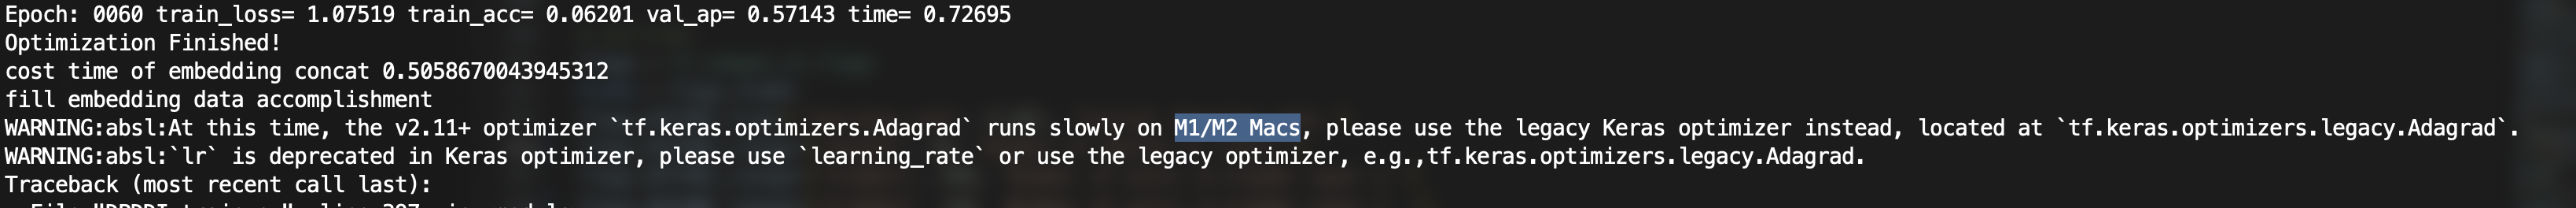
\includegraphics[width=0.9\linewidth]{fig/warning.png}
    \caption{Advertencia de ejecución lenta en chips de arquitectura ARM}
    \label{fig:warninr}
\end{figure}


\chapter{Apéndice: Documentación del código}

Debido a que el código actual no se encuentra adaptado para trabajar con versiones actuales de Python. se realizaron ajustes al mismo que se documentan a continuación:

\begin{figure}
    \centering
    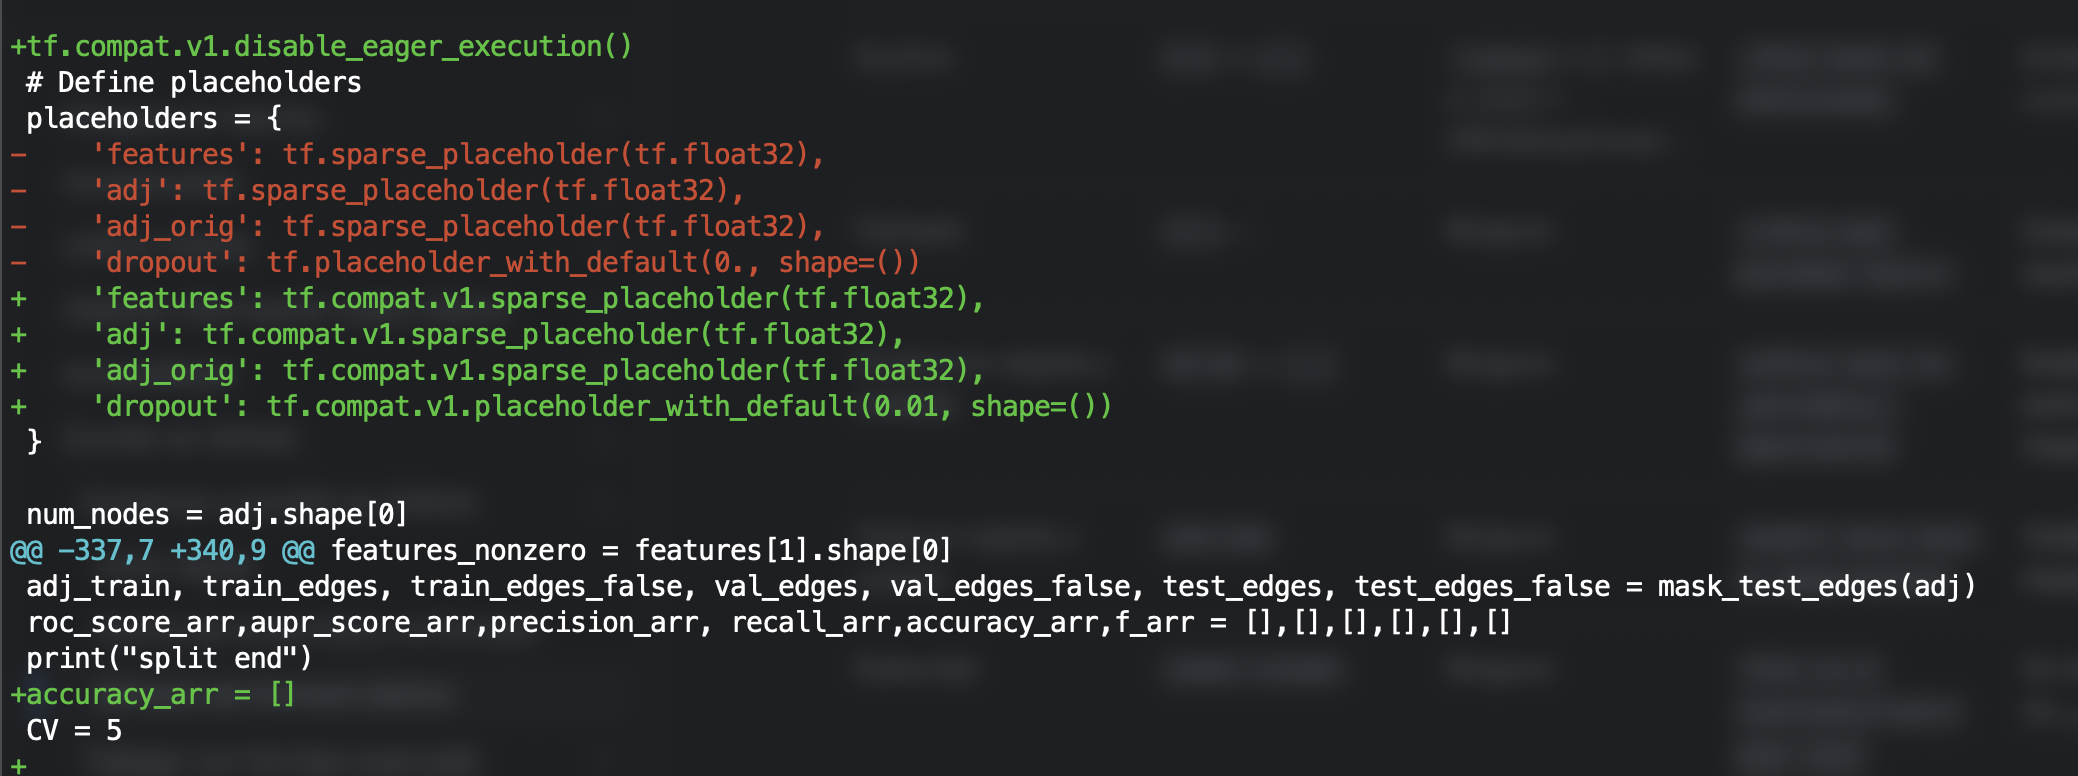
\includegraphics[width=1\linewidth]{fig/code_1.png}
    \caption{Modificación a la compatibilidad del sparse placeholder}
    \label{fig:enter-label}
\end{figure}

\begin{figure}
    \centering
    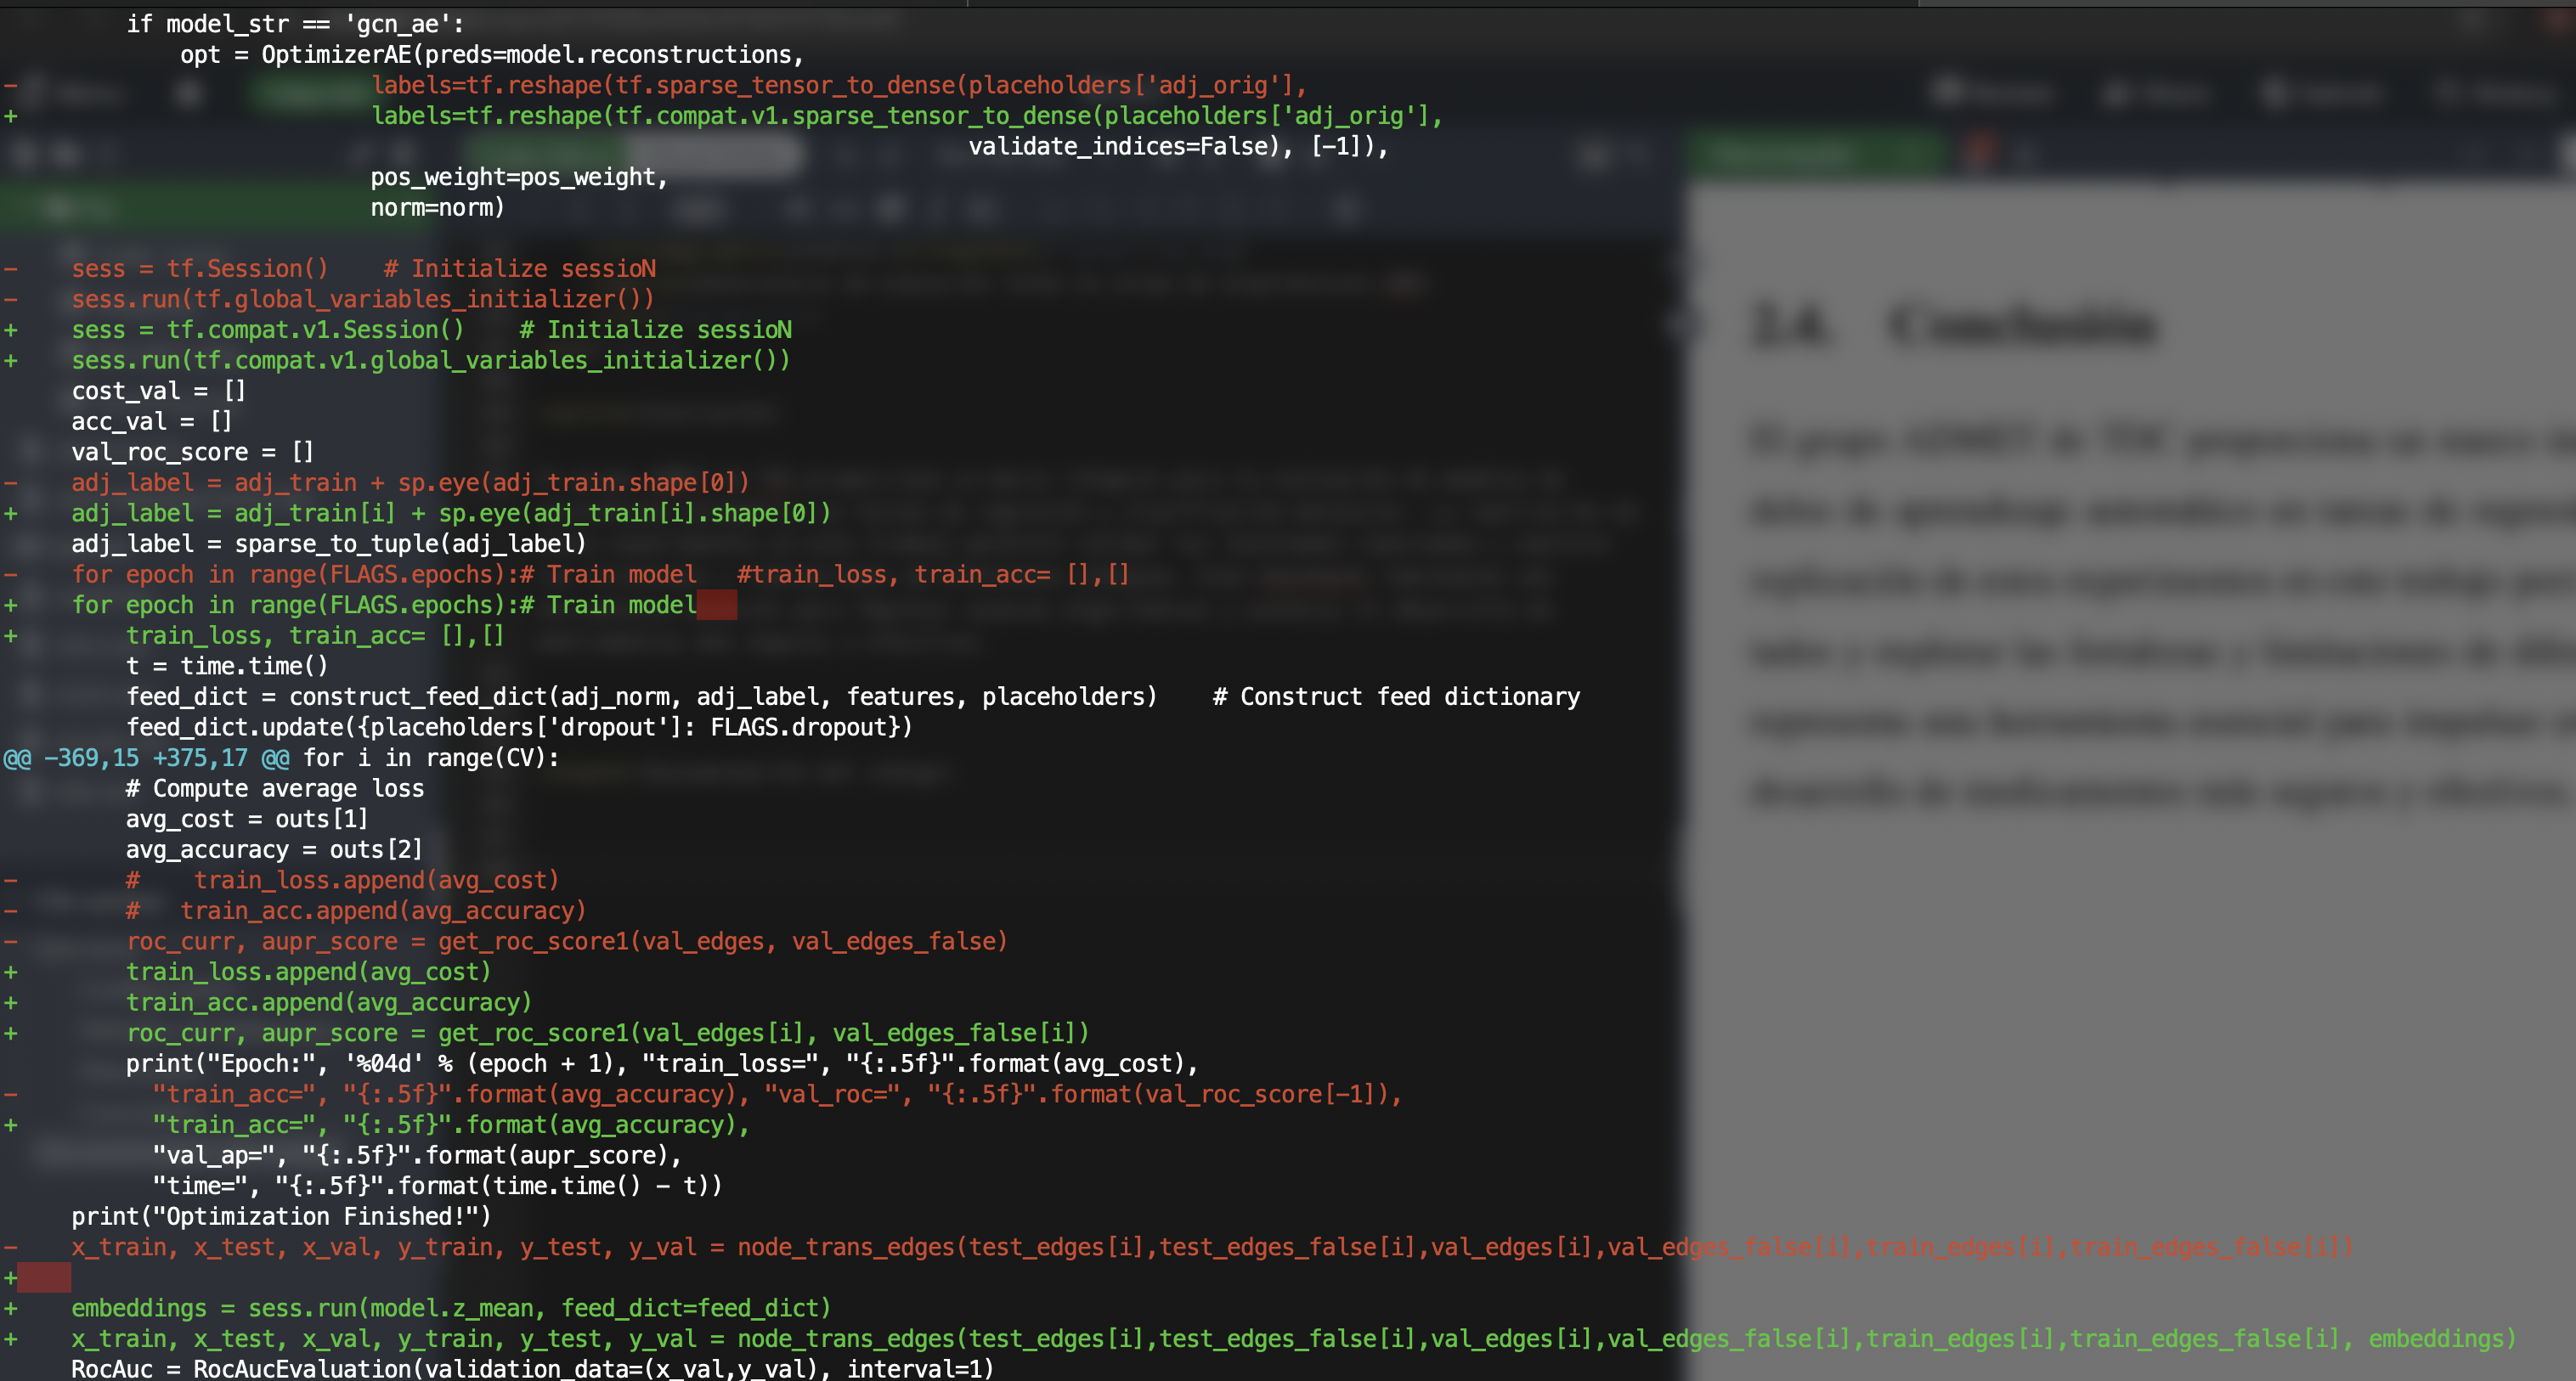
\includegraphics[width=1\linewidth]{fig/code2.png}
    \caption{Modificación a funciones de perdida y formateo de parámetros de accuracy}
    \label{fig:enter-label}
\end{figure}



\begin{figure}
    \centering
    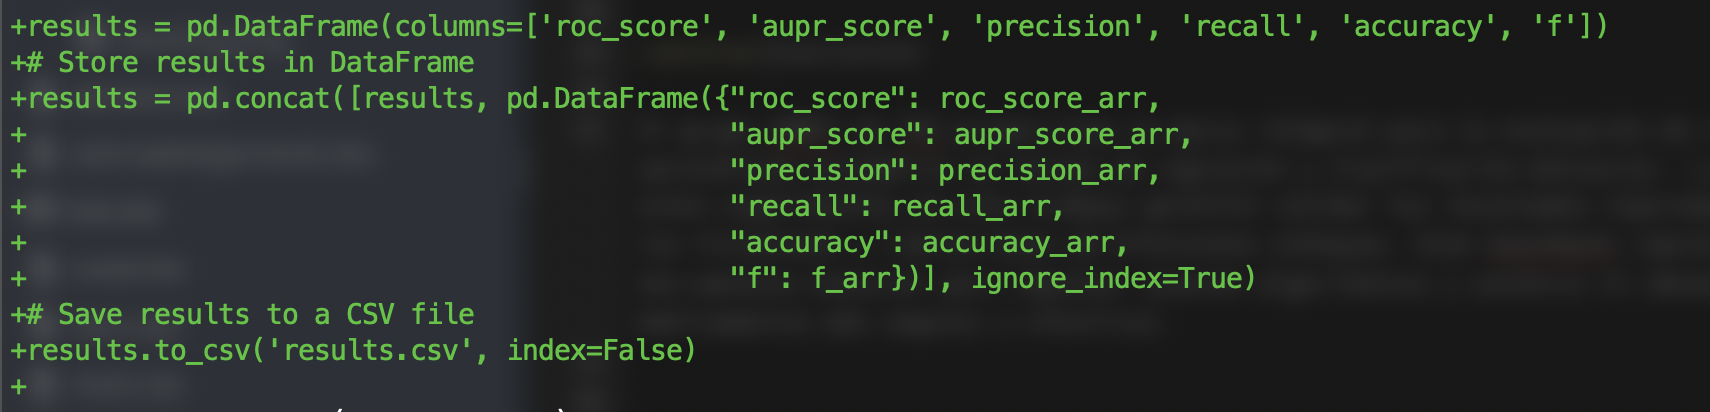
\includegraphics[width=1\linewidth]{fig/code3.png}
    \caption{Nuevo método implementado para almacenar resultados}
    \label{fig:enter-label}
\end{figure}


\begin{figure}
    \centering
    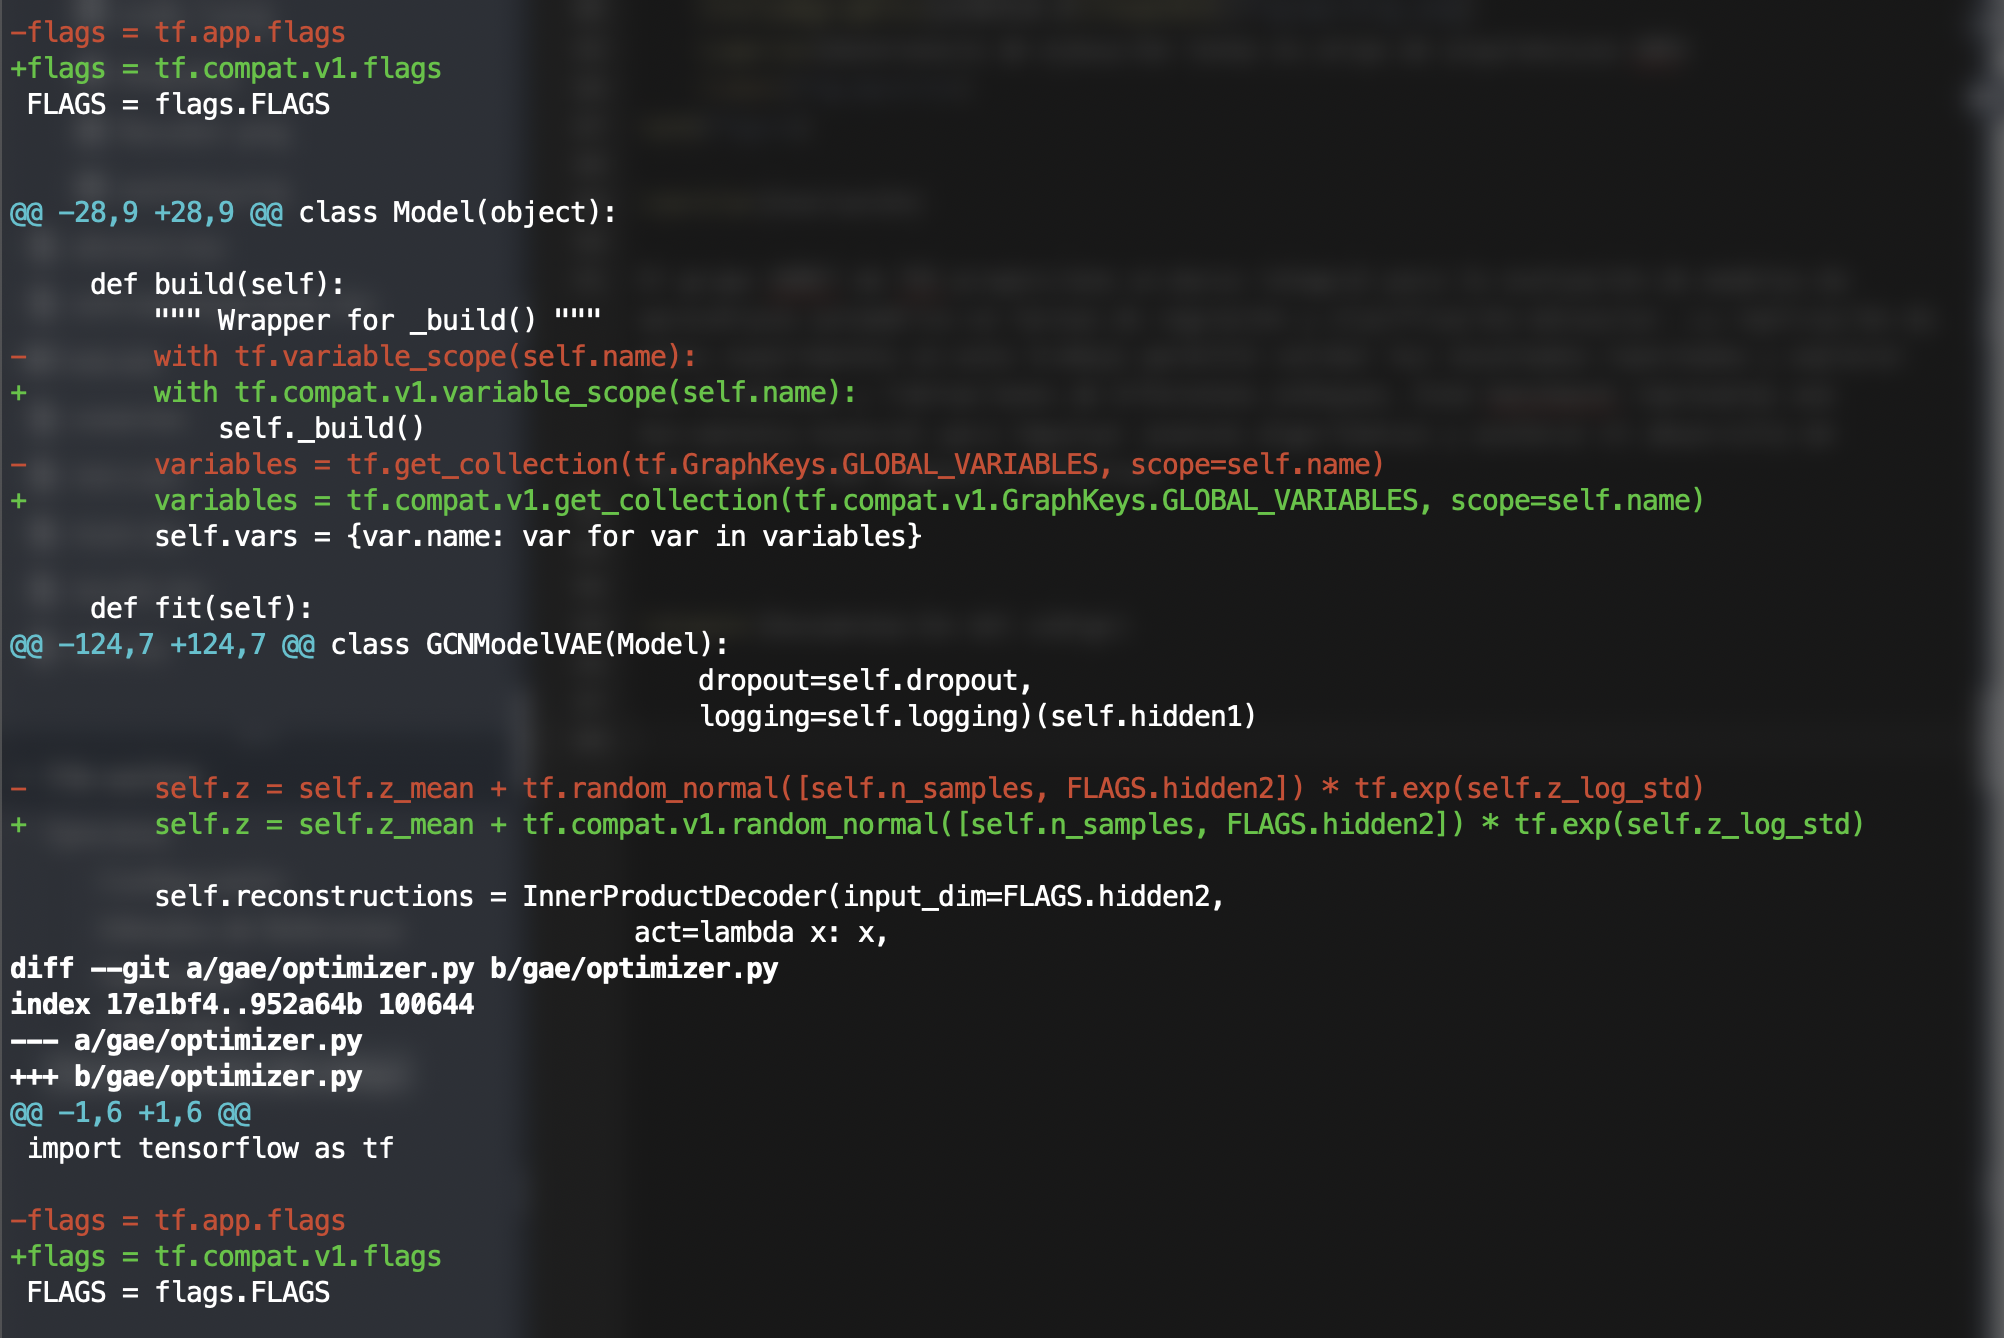
\includegraphics[width=1\linewidth]{fig/code4.png}
    \caption{Modificación a la forma de acceder a las variables flags en las rutinas}
    \label{fig:enter-label}
\end{figure}


\begin{figure}
    \centering
    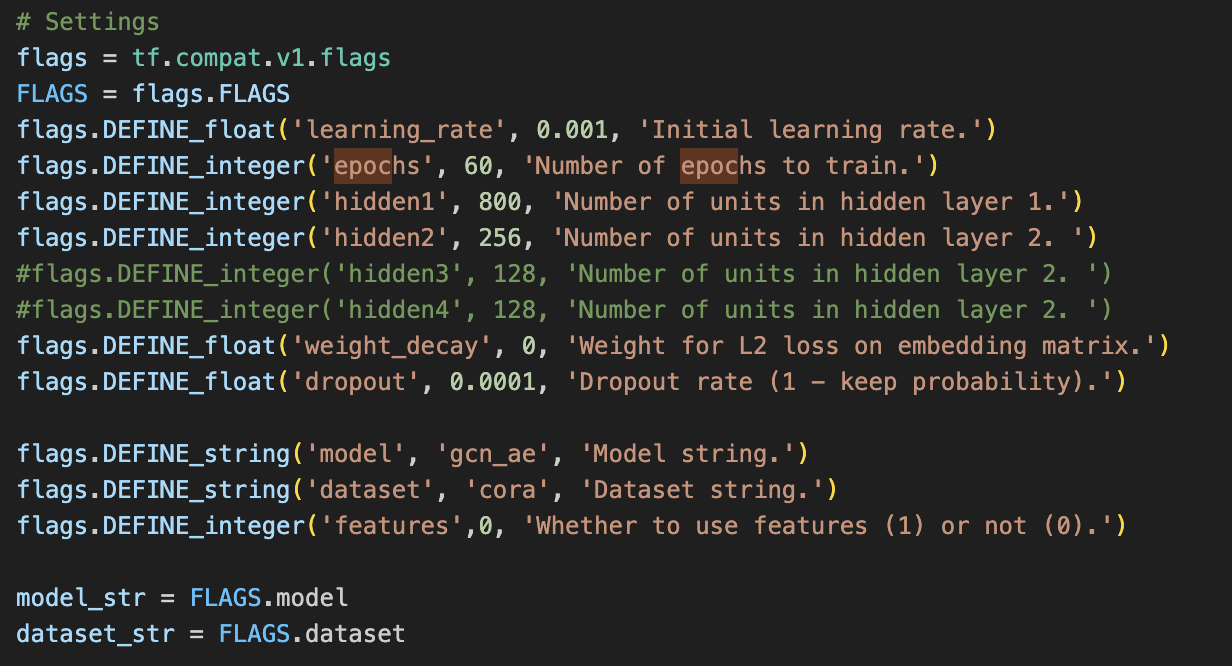
\includegraphics[width=1\linewidth]{fig/epoch.png}
    \caption{Modificación de cantidad de epocas para generar resultados en un tiempo viable
    }
    \label{fig:enter-label}
\end{figure}




\chapter{Benchmarking}

A continuación se presenta la tabla del ejercicio original realizado en el artículo \textbf{Benchmarking Molecular Machine Learning in Therapeutics Data Common}:
\begin{table}[ht]
\centering
\caption{Resultados en el grupo de benchmarks ADMET de TDC. Se reporta el promedio y la desviación estándar en cinco ejecuciones. Las flechas (↑, ↓) indican la dirección de mejor rendimiento. Los mejores métodos están en negritas y los segundos mejores están subrayados.}
\label{tab:admet_results}
\resizebox{\textwidth}{!}{%
\begin{tabular}{lcccccccc}
\toprule
\textbf{Dataset} & \textbf{Metric} & \textbf{Morgan} & \textbf{RDKit2D} & \textbf{CNN} & \textbf{NeuralFP} & \textbf{GCN} & \textbf{AttentiveFP} & \textbf{ContextPred} \\
\midrule
TDC.Caco2 (↓) & MAE & 0.908 ± 0.060 & 0.393 ± 0.024 & 0.446 ± 0.036 & 0.530 ± 0.102 & 0.599 ± 0.104 & 0.401 ± 0.032 & 0.502 ± 0.036 \\
TDC.HIA (↑) & AUROC & 0.807 ± 0.072 & 0.972 ± 0.008 & 0.869 ± 0.026 & 0.943 ± 0.014 & 0.936 ± 0.024 & 0.974 ± 0.007 & 0.975 ± 0.004 \\
TDC.Pgp (↑) & AUROC & 0.880 ± 0.006 & 0.918 ± 0.007 & 0.908 ± 0.012 & 0.902 ± 0.020 & 0.895 ± 0.021 & 0.892 ± 0.012 & 0.923 ± 0.005 \\
TDC.Bioav (↑) & AUROC & 0.581 ± 0.086 & 0.672 ± 0.021 & 0.613 ± 0.013 & 0.632 ± 0.036 & 0.566 ± 0.115 & 0.632 ± 0.039 & 0.671 ± 0.026 \\
TDC.Lipo (↓) & MAE & 0.701 ± 0.009 & 0.574 ± 0.017 & 0.743 ± 0.020 & 0.563 ± 0.023 & 0.541 ± 0.011 & 0.572 ± 0.007 & \textbf{0.535 ± 0.012} \\
TDC.AqSol (↓) & MAE & 1.203 ± 0.019 & 0.827 ± 0.047 & 1.023 ± 0.023 & 0.947 ± 0.016 & 0.907 ± 0.020 & 0.776 ± 0.008 & 1.040 ± 0.045 \\
TDC.BBB (↑) & AUROC & 0.823 ± 0.015 & 0.889 ± 0.016 & 0.781 ± 0.030 & 0.836 ± 0.009 & 0.842 ± 0.016 & 0.855 ± 0.011 & \textbf{0.897 ± 0.004} \\
TDC.PPBR (↓) & MAE & 12.848 ± 0.362 & 9.994 ± 0.319 & 11.106 ± 0.358 & 9.292 ± 0.384 & 10.194 ± 0.373 & 9.373 ± 0.335 & \underline{9.445 ± 0.224} \\
TDC.VD (↑) & Spearman & 0.493 ± 0.011 & 0.561 ± 0.025 & 0.226 ± 0.114 & 0.258 ± 0.162 & 0.457 ± 0.050 & 0.241 ± 0.145 & \underline{0.485 ± 0.092} \\
TDC.CYP2D6-I (↑) & AUPRC & 0.587 ± 0.011 & 0.616 ± 0.007 & 0.544 ± 0.053 & 0.627 ± 0.009 & 0.616 ± 0.020 & 0.646 ± 0.014 & \textbf{0.739 ± 0.005} \\
\bottomrule
\end{tabular}%
}
\end{table}
A continuación se presentan los resultados para la replicación de los resultados.


\begin{table}[ht]
\centering
\label{tab:admet_metrics}
\begin{tabular}{|l|c|c|}
\hline
\textbf{Dataset} & \textbf{Media} & \textbf{Desviación Estándar} \\ \hline
caco2\_wang & 0.932 & 0.061 \\ \hline
hia\_hou & 0.806 & 0.068 \\ \hline
pgp\_broccatelli & 0.878 & 0.010 \\ \hline
bioavailability\_ma & 0.553 & 0.094 \\ \hline
lipophilicity\_astrazeneca & 0.702 & 0.014 \\ \hline
solubility\_aqsoldb & 1.196 & 0.010 \\ \hline
bbb\_martins & 0.816 & 0.012 \\ \hline
ppbr\_az & 12.841 & 0.463 \\ \hline
vdss\_lombardo & 0.476 & 0.032 \\ \hline
cyp2d6\_veith & 0.582 & 0.013 \\ \hline
cyp3a4\_veith & 0.833 & 0.005 \\ \hline
cyp2c9\_veith & 0.719 & 0.008 \\ \hline
cyp2d6\_substrate\_carbonmangels & 0.669 & 0.036 \\ \hline
cyp3a4\_substrate\_carbonmangels & 0.638 & 0.011 \\ \hline
cyp2c9\_substrate\_carbonmangels & 0.382 & 0.011 \\ \hline
half\_life\_obach & 0.374 & 0.058 \\ \hline
clearance\_microsome\_az & 0.505 & 0.015 \\ \hline
clearance\_hepatocyte\_az & 0.270 & 0.069 \\ \hline
herg & 0.715 & 0.032 \\ \hline
ames & 0.801 & 0.009 \\ \hline
dili & 0.828 & 0.015 \\ \hline
ld50\_zhu & 0.642 & 0.020 \\ \hline
\end{tabular}
\caption{Resultados de los benchmarks ADMET con la red MORGAN con sus medias y desviaciones estándar.}
\end{table}

A continuación se muestran los resultados obtenidos directamente de la consola de ejecución:

\begin{figure}
    \centering
    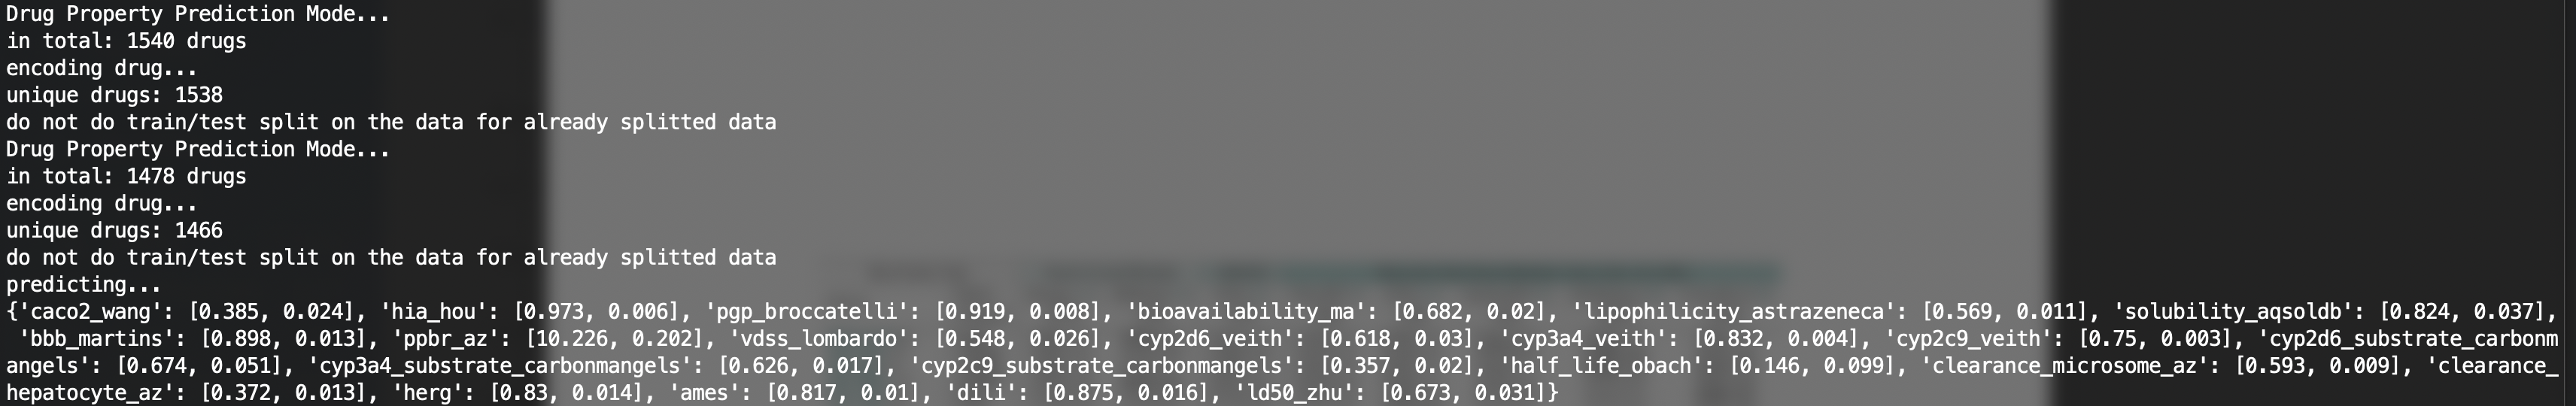
\includegraphics[width=1\linewidth]{fig/Results1.png}
    \caption{Ejecución de benchmark con red Morgan}
    \label{fig:enter-label}
\end{figure}
\printbibliography

\end{document}